\documentclass{article}
\usepackage{xcolor}
\usepackage[final]{../corl2027/corl_2026}

\usepackage{amsmath}
\usepackage{booktabs}
\usepackage{graphicx}
\usepackage{microtype}
\usepackage{hyperref}
\usepackage{tikz}
\usetikzlibrary{arrows.meta,positioning}
\raggedbottom

\title{WOD2ALPAsim:\\
Extending AlpaSim into a Closed-Loop Harness for WOD-Style Drivers}

\author{
  Alba Maria Tellez Fernandez\\
  \texttt{amtellezfernandez@gmail.com}
}

\begin{document}

\maketitle

\begin{abstract}
Closed-loop driving evaluation is often blocked by a practical but consequential mismatch:
datasets define one policy contract, while simulators execute another. The Waymo Open
Dataset end-to-end driving task exposes camera context, ego history, route intent, and a
fixed five-second trajectory target. AlpaSim executes native trajectory-model plugins
inside a simulator runtime with camera streams, ego dynamics, route updates, controller
execution, and deployment-specific service orchestration. This paper presents
WOD2ALPAsim, a full-stack adapter that made WOD-style and minimal-shot driving policies
run as AlpaSim external drivers. Although WOD is the motivating dataset contract, the
artifact also establishes a reusable adapter pattern for future AlpaSim integrations:
open only simulator-stable driver seams, reconstruct a compact policy signal outside
dataset-specific protobufs, register policies through the existing model-plugin
interface, and make deployment state executable through setup and launch scripts. The
artifact is not only a wrapper around policy code:
it patches the AlpaSim driver contract to pass route waypoints into model prediction,
hardens the driver service against late simulator messages, makes model imports lazy so
external plugins can load without heavyweight built-in backends, adds deploy/runtime
overrides for local external-driver execution, registers three project policies through
the \texttt{alpasim.models} plugin interface, reconstructs route and scene signals from
AlpaSim prediction inputs, and provides reproducible setup, readiness, and launch
scripts. This turns AlpaSim from a simulator that can run its built-in driver stack into
a harness for WOD-style trajectory policies, learned token policies, and actor-aware
planner variants under the same closed-loop runtime.
\end{abstract}

\keywords{autonomous driving, simulation, Waymo Open Dataset, closed-loop evaluation,
AlpaSim, policy adapters}

\section{Introduction}

The Waymo Open Dataset (WOD) end-to-end driving task is useful because it gives the
community a concrete policy interface: observe camera and ego context, condition on route
intent, and output a short-horizon ego trajectory~\citep{sun2020scalability}. That
interface is not the same thing as a simulator driver. AlpaSim is designed around live
closed-loop driver services and trajectory-model plugins~\citep{alpasim2026}. A
WOD-style policy can emit a trajectory, but AlpaSim expects a driver that can be
discovered as a model plugin, accept simulator-native camera and egomotion messages,
receive route updates, return headings and trajectory points at the configured rollout
clock, and survive the ordering behavior of a distributed simulator runtime.

The work in WOD2ALPAsim is therefore not "convert a log into a scene." The central
contribution is an execution bridge: we changed the AlpaSim-facing contract and the
project policy stack until WOD-style policies could be launched as first-class AlpaSim
external drivers. This required modifications on both sides of the boundary. On the
AlpaSim side, route waypoints had to be preserved beyond command classification and
passed through \texttt{PredictionInput}; model import had to tolerate local-driver
environments without Alpamayo or VAM installed; late close, image, egomotion, and route
messages had to be treated idempotently; and local external-driver deployment needed
repeatable Docker, wizard, and host-environment setup. On the policy side, our
minimal-shot, token-BC/DAgger, and direct actor-planner variants had to become native
AlpaSim model plugins while still preserving their WOD-style route, timing, and
trajectory assumptions.

The resulting artifact is a systems contribution suitable for a workshop because it
exposes a practical path from dataset-style policy development to closed-loop simulator
execution. More importantly, it sets a precedent for future AlpaSim adapters. The WOD
case reveals which seams need to be opened for external policies in general: route
geometry must survive into prediction, plugin discovery must not require unrelated
built-in model dependencies, distributed-runtime messages must be handled robustly, and
launch assumptions must be captured as executable state. The paper can therefore state
which parts are patched upstream AlpaSim, which parts are project-owned adapters, and
which runtime scripts make the result reproducible.

\paragraph{Contributions.}
We contribute:

\begin{enumerate}
  \item a comparison between stock AlpaSim's trajectory-driver contract and the contract
    needed by WOD-style policies;
  \item AlpaSim-side patches that expose route waypoints to model prediction, support
    dependency-light external plugins, harden asynchronous driver sessions, and adapt
    local deployment;
  \item project-side AlpaSim model plugins for a minimal-shot reflex policy, a learned
    token BC/DAgger policy, and a selector-free actor-aware planner;
  \item a signal reconstruction layer that turns AlpaSim prediction inputs into route,
    dynamics, visibility, and optional actor/hazard context; and
  \item a reusable adapter pattern for future AlpaSim bridges, with a reproducible setup
    and launch path that installs the local plugin into an AlpaSim checkout, verifies
    registry discovery, writes matched driver/wizard commands, runs named scene presets,
    and checks artifact invariants through unit tests and readiness scripts.
\end{enumerate}

\section{Why a Thin Adapter Was Not Enough}

Stock AlpaSim already has the right high-level architecture for this task: a runtime
queries an ego-driver service, the driver returns a trajectory, and downstream controller
and vehicle components execute it. The mismatch appeared in the details of the driver
contract and deployment path. Table~\ref{tab:stock_vs_adapted} summarizes the difference.

\begin{table}[t]
\centering
\small
\begin{tabular}{p{0.23\linewidth}p{0.31\linewidth}p{0.34\linewidth}}
\toprule
Surface & Stock AlpaSim behavior & WOD2ALPAsim behavior \\
\midrule
Route input & route used mainly for command & route waypoints preserved for prediction \\
Model imports & eager built-in backend imports & lazy imports for external plugin envs \\
Plugin boundary & built-in model stack & local \texttt{alpasim.models} policies \\
Session messages & unknown-session errors & late messages handled idempotently \\
Trajectory output & simulator frequency contract & WOD-style 5 s horizon resampled to runtime \\
Deployment & wizard-driven built-ins & matched external driver and wizard commands \\
Host setup & monolithic dependency assumptions & minimal editable install and overrides \\
\bottomrule
\end{tabular}
\caption{The adapter changes both the AlpaSim-side execution surface and the
project-side policy surface.}
\label{tab:stock_vs_adapted}
\end{table}

The most important issue was route information. In the original driver API,
\texttt{PredictionInput} contained camera images, command, speed, acceleration, and ego
pose history. That is enough for a command-conditioned model, but not for policies that
need the local route geometry. WOD2ALPAsim stores the latest route submitted by the
runtime, copies its waypoints into \texttt{PredictionInput}, and lets model plugins build
a local route centerline from simulator waypoints. This is a small patch in code size and
a large change in capability: policies can now reason over the actual AlpaSim route
instead of only a left/straight/right symbol.

The second issue was plugin loading. A local external-driver environment may not contain
every heavy dependency needed by AlpaSim's built-in learned models. Eagerly importing all
built-ins blocks unrelated external plugins. WOD2ALPAsim replaces that import path with
lazy loading: the base abstractions remain importable, the manual model remains
available, and heavy built-ins load only if explicitly requested. That lets our policies
register through \texttt{alpasim.models} without carrying the entire built-in driver
dependency stack.

The third issue was runtime robustness. In a service-oriented simulator, messages can
arrive after a session has closed or after another service has already advanced. The
patched driver treats duplicate closes and late image, egomotion, and route updates as
warnings instead of fatal errors. This does not change the driving policy; it makes batch
rollouts practical.

Figure~\ref{fig:contract_patch} shows the concrete driver-contract change. The stock
path classifies route updates into a compact command and sends that command to the model.
The patched path still preserves the command, but also passes route waypoints, ego
dynamics, camera context, and pose history into the external plugin. This is the minimum
opening needed for WOD-style policies to reason about route geometry without becoming
AlpaSim-internal code.

\begin{figure}[t]
\centering
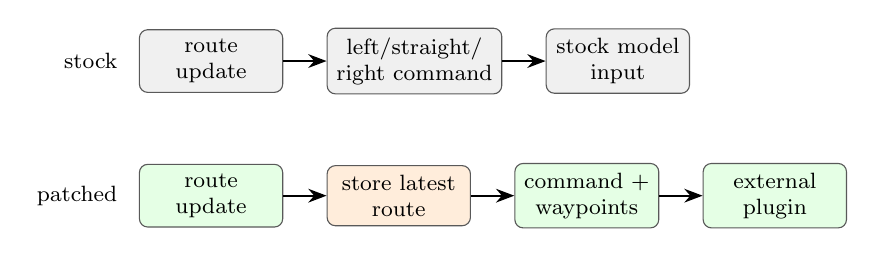
\begin{tikzpicture}[
  node distance=0.5cm and 0.55cm,
  box/.style={rectangle,rounded corners=3pt,draw=black!65,minimum height=0.62cm,
              minimum width=1.82cm,font=\footnotesize,align=center},
  stock/.style={box,fill=gray!12},
  patched/.style={box,fill=green!10},
  seam/.style={box,fill=orange!14},
  arr/.style={-Stealth,thick}
]
  \node[stock] (route_a) {route\\update};
  \node[stock,right=of route_a] (cmd_a) {left/straight/\\right command};
  \node[stock,right=of cmd_a] (model_a) {stock model\\input};

  \node[patched,below=0.9cm of route_a] (route_b) {route\\update};
  \node[seam,right=of route_b] (store_b) {store latest\\route};
  \node[patched,right=of store_b] (input_b) {command +\\waypoints};
  \node[patched,right=of input_b] (plugin_b) {external\\plugin};

  \draw[arr] (route_a) -- (cmd_a);
  \draw[arr] (cmd_a) -- (model_a);
  \draw[arr] (route_b) -- (store_b);
  \draw[arr] (store_b) -- (input_b);
  \draw[arr] (input_b) -- (plugin_b);

  \node[font=\footnotesize,align=right,left=0.15cm of route_a] {stock};
  \node[font=\footnotesize,align=right,left=0.15cm of route_b] {patched};
\end{tikzpicture}
\caption{The key AlpaSim driver-contract patch preserves route waypoints for prediction
instead of reducing route input to a command-only signal.}
\label{fig:contract_patch}
\end{figure}

\section{Adapter Architecture}

Figure~\ref{fig:architecture} shows the implemented architecture. The bridge has two
layers: AlpaSim-side enablement and policy-side adaptation.

\begin{figure}[t]
\centering
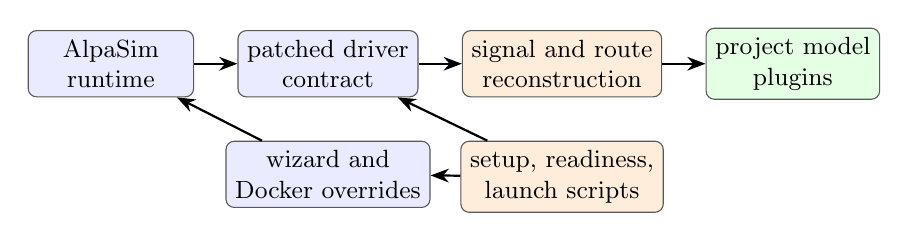
\begin{tikzpicture}[
  node distance=0.55cm and 0.55cm,
  box/.style={rectangle,rounded corners=3pt,draw=black!65,minimum height=0.72cm,
              minimum width=2.1cm,font=\small,align=center},
  alpa/.style={box,fill=blue!8},
  bridge/.style={box,fill=orange!14},
  pol/.style={box,fill=green!10},
  arr/.style={-Stealth,thick}
]
  \node[alpa] (runtime) {AlpaSim\\runtime};
  \node[alpa,right=of runtime] (driver) {patched driver\\contract};
  \node[bridge,right=of driver] (signal) {signal and route\\reconstruction};
  \node[pol,right=of signal] (models) {project model\\plugins};
  \node[bridge,below=of signal] (launch) {setup, readiness,\\launch scripts};
  \node[alpa,below=of driver] (wizard) {wizard and\\Docker overrides};

  \draw[arr] (runtime) -- (driver);
  \draw[arr] (driver) -- (signal);
  \draw[arr] (signal) -- (models);
  \draw[arr] (launch) -- (driver);
  \draw[arr] (launch) -- (wizard);
  \draw[arr] (wizard) -- (runtime);
\end{tikzpicture}
\caption{WOD2ALPAsim is a full-stack integration: patched AlpaSim driver and deployment
surfaces feed project-owned model plugins through a reconstructed policy signal.}
\label{fig:architecture}
\end{figure}

\subsection{AlpaSim-Side Enablement}

The patched AlpaSim checkout contains four relevant changes.

\paragraph{Route waypoint propagation.}
The driver session now stores the most recent route and exposes it through
\texttt{route\_waypoints\_for\_prediction}. The batch prediction path copies those
waypoints into \texttt{PredictionInput}. This preserves the route geometry generated by
AlpaSim's runtime and makes it available to every external model plugin.

\paragraph{Dependency-light model registry.}
The model package keeps \texttt{BaseTrajectoryModel}, \texttt{PredictionInput},
\texttt{ModelPrediction}, \texttt{DriveCommand}, and \texttt{ManualModel} importable
without importing all heavyweight backends. Alpamayo and VAM remain available through
lazy access when installed. External plugins therefore need only the base driver
abstractions.

\paragraph{Asynchronous session hardening.}
The driver now handles unknown-session close, image, egomotion, and route messages as
late or duplicate messages rather than immediate crashes. This matters for long batch
runs where the simulator, driver, controller, and renderer do not always stop at exactly
the same microsecond.

\paragraph{Local external-driver deployment.}
The override layer adds deployment and Docker changes for local external-driver use,
including host/wizard command generation, ARM-aware deploy selection, minimal Docker
dependency groups, and GPU reservation behavior that matches local topologies. The point
is not to claim a new simulator backend; it is to make the external-driver path runnable
without hand-editing AlpaSim configuration for every experiment.

\subsection{Policy-Side Adaptation}

The project registers three AlpaSim model entry points:
\texttt{spotlight\_reflex}, \texttt{token\_dagger\_bc}, and
\texttt{direct\_actor\_planner}. Each implements AlpaSim's
\texttt{BaseTrajectoryModel.from\_config} factory and returns
\texttt{ModelPrediction} objects with trajectory points, headings, and structured
reasoning metadata.

\paragraph{Minimal-shot reflex plugin.}
The reflex adapter maps AlpaSim's \texttt{DriveCommand} to the policy's route command,
extracts route and scene signal, evaluates maneuver candidates, applies route-stability
constraints, resamples the selected trajectory to the configured output frequency, and
returns headings.

\paragraph{Token BC/DAgger plugin.}
The learned adapter loads token-policy checkpoints, normalizes geometric features,
supports multiple selection modes, and can combine learned logits with route, lane,
static-clearance, and actor-clearance constraints. It also supports clamped lateral
geometry, hybrid veto modes, actor-axis modes, and per-run selection logs.

\paragraph{Direct actor-planner plugin.}
The selector-free planner bypasses token logits and samples a small continuous trajectory
family. It scores candidates with actor, route, lane, smoothness, progress, speed, and
rear-flow terms, then returns the best trajectory under the same AlpaSim driver contract.
This makes the harness useful for comparing tokenized and direct planning interfaces
inside one simulator.

\section{Audited Artifact Surface}

The implementation is deliberately split into patched upstream AlpaSim surface area and
project-owned adapter surface area. Table~\ref{tab:artifact_surface} lists the core
surfaces because this is the main evidence that the contribution is more than a wrapper.

\begin{table}[t]
\centering
\small
\begin{tabular}{p{0.31\linewidth}p{0.58\linewidth}}
\toprule
Surface & Implemented role \\
\midrule
\texttt{alpasim\_driver.models.base} &
Extends \texttt{PredictionInput} with route waypoints so plugins receive route geometry. \\
\texttt{alpasim\_driver.main} &
Stores submitted routes, forwards route waypoints into batch prediction, and treats late
session messages idempotently. \\
\texttt{alpasim\_driver.models} &
Uses lazy built-in model imports so external plugins can load in dependency-light driver
environments. \\
Wizard and Docker overrides &
Adapt local external-driver deployment, host networking, GPU reservations, and minimal
runtime dependencies. \\
\texttt{alpasim\_signal.py} &
Reconstructs route, dynamics, visibility, static hazards, and moving actors from
AlpaSim prediction inputs. \\
\texttt{alpasim\_spotlight.py} &
Wraps the minimal-shot reflex policy as a native AlpaSim trajectory model. \\
\texttt{alpasim\_token\_bc.py} &
Runs learned token BC/DAgger checkpoints with route, lane, actor, and hybrid-veto
selection modes. \\
Direct planner adapter &
Runs a selector-free actor-aware trajectory sampler under the same driver contract. \\
Setup and launch commands &
Apply overrides, bootstrap the AlpaSim environment, verify \texttt{alpasim.models}
discovery, check runtime readiness, and emit reproducible driver/wizard commands. \\
\bottomrule
\end{tabular}
\caption{Audited implementation surfaces. The bridge required both patched AlpaSim code
and project-owned model adapters.}
\label{tab:artifact_surface}
\end{table}

\section{Artifact Contents}

The artifact is organized as a reproducible integration bundle rather than a single
script. Table~\ref{tab:artifact_contents} lists the bundle components and the claim each
component supports. This is the checklist a reviewer should use to distinguish the
adapter from ordinary experiment glue.

\begin{table}[t]
\centering
\small
\begin{tabular}{p{0.33\linewidth}p{0.56\linewidth}}
\toprule
Bundle component & Reviewer-visible purpose \\
\midrule
AlpaSim overrides &
Tracks the replacement files under \texttt{third\_party/alpasim\_overrides}: the
route-waypoint propagation patch, lazy model imports, and deployment overrides. \\
Driver configs &
Defines native AlpaSim driver YAMLs for the reflex, token BC/DAgger, and direct
actor-planner plugins. \\
Setup command &
Applies overrides, bootstraps the AlpaSim environment, installs editable packages, and
checks model entry-point discovery. \\
Readiness command &
Checks the non-code runtime assumptions: checkout shape, Docker access, GPU runtime,
base image, platform constraints, and scene artifacts. \\
External-run launcher &
Materializes matched driver/wizard commands and launch metadata before optional
closed-loop execution. \\
AlpaSim tests &
Verifies plugin registration, signal reconstruction, adapter outputs, checkpoint
compatibility, override application, setup planning, and launch command generation. \\
\bottomrule
\end{tabular}
\caption{Artifact bundle contents. Each component supports a concrete integration claim
that can be inspected independently of the final closed-loop rollout.}
\label{tab:artifact_contents}
\end{table}

\section{Signal Reconstruction}

The adapter reconstructs a compact policy scenario from \texttt{PredictionInput}. It
extracts route waypoints from the patched AlpaSim field when present, falling back to a
command-proxy route only when route geometry is unavailable. It also extracts speed,
acceleration, pose-history length, camera count, a simple visibility-risk signal from
camera brightness, and optional structured hazards from fields such as
\texttt{structured\_hazards}, \texttt{hazards}, \texttt{traffic\_hazards}, or
\texttt{alpasignal}.

Structured hazards are converted into the internal policy representation. Static hazards
become obstacles with shape and heading metadata. Moving hazards become actors with
velocity, size, heading, and inferred or explicit behavior. Route waypoints become the
local lane centerline used by the policy and planner. If no explicit hazard is available
but visibility or dynamics indicate a high-risk state, the adapter can add a caution-zone
obstacle. This layer is intentionally independent of WOD protobufs and AlpaSim internals:
it is the stable policy-facing signal produced by the bridge.

\section{Reproducible Execution Path}

The integration includes scripts that make the bridge repeatable rather than anecdotal.
The setup command validates that \texttt{ALPASIM\_ROOT} is a real checkout, applies
repo-tracked AlpaSim patches and overrides, bootstraps the AlpaSim virtual environment,
compiles protobuf modules, installs the required AlpaSim packages editably, installs this
repository as a no-dependency editable package, and verifies that the required
\texttt{alpasim.models} entry points are discoverable.

The readiness command checks the AlpaSim checkout shape, Docker access, platform
compatibility, the local AlpaSim base image, NVIDIA container runtime visibility, and
scene artifacts. The run launcher then materializes an
\texttt{external-driver-config.yaml}, \texttt{driver-command.sh},
\texttt{wizard-command.sh}, and \texttt{launch-metadata.json}. It supports named scene
presets and policy presets, including learned checkpoint variants and actor-aware
planner variants. The driver and wizard are launched as a matched pair: the driver runs
from the AlpaSim virtual environment, while the wizard receives the external driver
address, topology, scene IDs, log directory, base port, and timeout.

This matters because AlpaSim experiments otherwise depend on a fragile mixture of Hydra
overrides, Docker image state, plugin installation state, gated scene artifacts, and
host-specific GPU behavior. WOD2ALPAsim makes those assumptions explicit.

\section{Artifact Validation}

The artifact is organized around invariants that can be checked without reading the
entire simulator. Table~\ref{tab:artifact_validation} lists the reviewer-facing checks.
They are not performance claims; they are integration claims that establish the bridge is
usable and inspectable.

\begin{table}[t]
\centering
\small
\begin{tabular}{p{0.36\linewidth}p{0.53\linewidth}}
\toprule
Invariant & Artifact check \\
\midrule
Local policies are discoverable by AlpaSim &
The package registers \texttt{spotlight\_reflex}, \texttt{token\_dagger\_bc}, and
\texttt{direct\_actor\_planner} under \texttt{alpasim.models}; setup verifies registry
discovery in the AlpaSim virtual environment. \\
Route geometry reaches policy code &
Signal tests construct prediction inputs with route waypoints and verify that the
resulting policy scenario uses \texttt{alpasim\_waypoints} as its route source. \\
Scene signal is policy-facing, not protobuf-facing &
Tests pass structured hazards through multiple input aliases and verify static
obstacles, moving actors, shape metadata, headings, velocities, and inferred behaviors. \\
Adapters satisfy the trajectory-model contract &
The reflex, token BC/DAgger, and direct planner adapters return trajectory arrays,
headings, and structured reasoning payloads through the AlpaSim model API. \\
Learned-policy checkpoints are contract-checked &
Token-policy loading verifies token names, feature normalizers, device selection, and
selection-log outputs; bad token schemas are rejected. \\
Setup and launch are reproducible &
Setup-script tests cover checkout validation, override application, protobuf
compilation, editable install planning, driver command generation, wizard command
generation, scene preset loading, Docker/image preflights, and platform guards. \\
\bottomrule
\end{tabular}
\caption{Artifact validation targets integration invariants: plugin discovery, route
propagation, signal reconstruction, model contract compliance, checkpoint compatibility,
and reproducible launch state.}
\label{tab:artifact_validation}
\end{table}

The minimal reviewer path is therefore concrete. First, run the setup command in
check-only mode to verify that the AlpaSim checkout can see the local model entry points.
Second, run the readiness command to check Docker, GPU runtime, scene artifacts, and
platform assumptions. Third, launch in print mode to materialize the exact driver and
wizard commands without starting a rollout. Finally, run the AlpaSim integration and
setup-script tests to verify the adapter invariants above. This gives reviewers a
bounded artifact audit: if any of these checks fails, the bridge contract is broken in a
specific place.

Figure~\ref{fig:artifact_path} summarizes this audit path. The point is that the
artifact is not validated by a single successful rollout. It is validated by a sequence of
checks that isolate whether failures come from patch application, plugin discovery,
runtime prerequisites, launch materialization, or adapter semantics.

\begin{figure}[t]
\centering
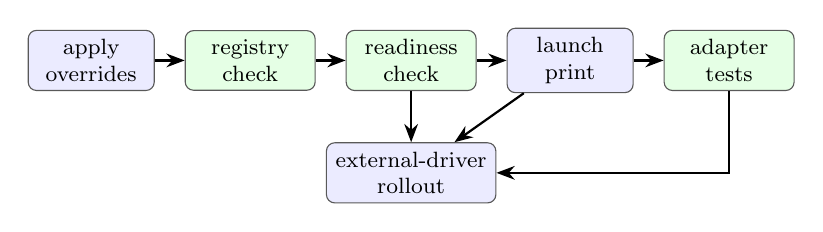
\begin{tikzpicture}[
  node distance=0.45cm and 0.38cm,
  auditstep/.style={rectangle,rounded corners=3pt,draw=black!65,fill=blue!8,
               minimum height=0.66cm,minimum width=1.6cm,font=\footnotesize,align=center},
  check/.style={rectangle,rounded corners=3pt,draw=black!65,fill=green!10,
               minimum height=0.66cm,minimum width=1.65cm,font=\footnotesize,align=center},
  arr/.style={-Stealth,thick}
]
  \node[auditstep] (overrides) {apply\\overrides};
  \node[check,right=of overrides] (registry) {registry\\check};
  \node[check,right=of registry] (ready) {readiness\\check};
  \node[auditstep,right=of ready] (print) {launch\\print};
  \node[check,right=of print] (tests) {adapter\\tests};

  \node[auditstep,below=0.65cm of ready] (rollout) {external-driver\\rollout};

  \draw[arr] (overrides) -- (registry);
  \draw[arr] (registry) -- (ready);
  \draw[arr] (ready) -- (print);
  \draw[arr] (print) -- (tests);
  \draw[arr] (ready) -- (rollout);
  \draw[arr] (print) -- (rollout);
  \draw[arr] (tests) |- (rollout);
\end{tikzpicture}
\caption{Reviewer-facing artifact path. Setup, readiness, command materialization, and
tests isolate integration failures before expensive closed-loop rollouts.}
\label{fig:artifact_path}
\end{figure}

\section{What the Adapter Enables}

The artifact enables three concrete workflows and one broader engineering precedent.

\paragraph{Closed-loop execution of WOD-style policies.}
Policies developed around WOD-style route, timing, and trajectory conventions can run as
AlpaSim external drivers. The simulator repeatedly queries the plugin and executes the
returned trajectory through its controller path.

\paragraph{Shared runtime for heterogeneous policies.}
The reflex policy, learned token policy, and direct actor planner share one driver
contract, one route signal, one trajectory resampling path, and one launch system. This
lets policy-interface questions be tested inside a single closed-loop runtime rather than
through separate bespoke scripts.

\paragraph{Inspectable transfer infrastructure.}
Because the bridge separates patched upstream work from project-owned adapters, it is
clear which claims depend on AlpaSim modifications and which depend on policy logic. That
separation is useful for workshop review: the contribution can be audited as an artifact,
not merely described as a conceptual adapter.

\paragraph{A precedent for future AlpaSim adapters.}
The same pattern can support future bridges for other dataset or benchmark contracts:
preserve simulator-native route geometry at the driver boundary, avoid dataset protobufs
inside policy code, expose only compact policy-facing signal, keep policies registered as
ordinary AlpaSim model plugins, and make setup plus launch assumptions executable. In
this sense, WOD2ALPAsim is both a WOD bridge and a reference pattern for building
additional AlpaSim adapters.

\section{Limitations}

WOD2ALPAsim does not claim to reconstruct the full WOD world state inside AlpaSim. Its
primary claim is execution compatibility: making WOD-style and project policies run as
native AlpaSim drivers. Richer traffic reconstruction, broader WOD subset release,
dataset-terms packaging, and standard public baselines are natural next steps. The
current artifact already exposes the important systems boundary: route geometry,
trajectory timing, plugin loading, deployment, and simulator-driver interaction.

\section{Conclusion}

WOD2ALPAsim is a full-stack adapter, not a thin wrapper. The work patched AlpaSim's
driver input contract, deployment path, and import behavior; registered project policies
as AlpaSim model plugins; reconstructed route and scene signal for WOD-style policies;
and added reproducible setup, readiness, and launch tooling. The result is a practical
closed-loop harness for running minimal-shot, learned token, and actor-aware planning
policies under AlpaSim's simulator runtime. That is the workshop contribution: the
engineering bridge pattern that turns dataset-style trajectory policies into executable
closed-loop drivers. Future AlpaSim adapters should be built at stable driver, signal,
plugin, and launch seams rather than as one-off simulator forks or dataset-specific
policy rewrites.

\bibliography{paper}

\end{document}
